%%% Uppsala University presentation beamer template v2.0
%%% provided by Diletta Goglia, IT Department, Uppsala University
%%% email: diletta.goglia@it.uu.se
%%% December, 2023

% This template is the updated version of the "Uppsala University presentation template v1.0" created by Mats Jonsson (mats@mekeriet.se) in March 2021.


\documentclass{beamer}

\usepackage[english]{babel}
\usepackage[utf8x]{inputenc}
\usepackage{hyperref, % clickable links
    graphicx, % include images
    listings, % for code and formatting
    caption, % customization of captions in figures and tables
    stackengine, % custom layouts 
    amsmath, % math env
    xcolor, % extend color support
    multicol, % multiple columns layout
    booktabs, % high quality tables
    lipsum % remove it
}

\usepackage{UU_beamer} % customized style
\usefonttheme[onlymath]{serif}

\def\cmd#1{\texttt{\color{red}\footnotesize $\backslash$#1}}
\def\env#1{\texttt{\color{blue}\footnotesize #1}}

% ------ CODE COLOR DEFINITION ------ %

\definecolor{codered}{rgb}{0.6,0,0}
\definecolor{codeblue}{rgb}{0,0,0.8}
\definecolor{codegreen}{rgb}{0,0.5,0}
\definecolor{almostwhite}{gray}{0.55}
\definecolor{codepurple}{rgb}{0.58,0,0.82}
\definecolor{backcolour}{rgb}{0.95,0.95,0.92}

\lstset{
    basicstyle=\ttfamily\small,
    keywordstyle=\bfseries\color{codeblue},
    emphstyle=\ttfamily\color{codered},   % Custom highlighting style
    stringstyle=\color{codepurple},
    numbers=left,
    numberstyle=\small\color{almostwhite},
    rulesepcolor=\color{red!20!green!20!blue!20},
    frame=shadowbox,
    commentstyle=\color{codegreen},
    captionpos=b    
}

% ------------- PRESENTATION INFO --------------- %
\newcommand{\fullconference}{Presentation}
\newcommand{\shortconference}{}
\newcommand{\contact}{\textit{vincent.dahlberg@gmail.com \\ a3iskasson@outlook.com}}

\author[V. Dahlberg, A. Roos Isaksson, \contact]{\href{}{Vincent Dahlberg, Albin Roos Isaksson}}
\institute[IT Dep, UU]{\href{}{IT Department, Uppsala University}
    \\ \smallskip \contact}
\title[SR to Analyse Toeplitz]{Symbolic Regression to Analyse Toeplitz matrices}
\subtitle[\shortconference]{Unearthing Spectral Truths with Symbolic Regression}
\date[June 2025]{\small \today
    \\ \fullconference}


\begin{document}

% ------------ TITLE SLIDE --------------- %
{
% Remove headline and footline from first slide
\setbeamertemplate{footline}{} 
\setbeamertemplate{headline}{} 

\begin{frame}\label{start}
    \titlepage
    \begin{figure}
            
\includegraphics[scale=0.65]{style/uu_logo.pdf} 
    \end{figure}
\end{frame}
}

% ---------- TABLE OF CONTENT --------- %
\begin{frame}{Agenda}
    \tableofcontents[sectionstyle=show, subsectionstyle=show/shaded/hide, subsubsectionstyle=show/shaded/hide]
\end{frame}


\section{Introduktion}

\begin{frame}{Toeplitz matriser}
En Toeplitz matris är en matris med konstanta diagonala element. Exempel: Diskreta Laplace operatorn med andra ordningens finita differenser.
    \begin{equation}
        -\Delta = \begin{bmatrix}
        2 & -1 &  &  0\\
        -1 & \ddots & \ddots &  \\
         & \ddots & \ddots & -1 \\
         0& & -1 & 2
    \end{bmatrix}
    \end{equation}
\end{frame}


\begin{frame}{Toeplitz matriser och genererande symboler}
    Man kan relatera en Toeplitz matris $T_n$ med en s.k. \textit{generating symbol} $f$, där $f$ är en Fourierserie där koefficienterna är matrisens element.
\begin{equation}
    T_n(f) = \begin{bmatrix}
    \hat{\mathnormal{f}}_0&\hat{\mathnormal{f}}_{-1}& \cdots &\hat{\mathnormal{f}}_{-(n-1)} \\
     \hat{\mathnormal{f}}_{1}&  \hat{\mathnormal{f}}_0& \ddots &\vdots\\
    \vdots& \ddots& \ddots& \hat{\mathnormal{f}}_{-1} \\
     \hat{\mathnormal{f}}_{n-1}&\cdots& \hat{\mathnormal{f}}_{1}& \hat{\mathnormal{f}}_0
\end{bmatrix}, \quad\quad f(\theta) = \sum^\infty_{k = -\infty} \hat{\mathnormal{f}}_k e^{\mathbf{i}k\theta}
\end{equation}
Formellt säger man att $f$ genererar $T_n(f)$.
\end{frame}


\begin{frame}{Exempel: Symboler}
    Vi återgår till exemplet där $T$ är $10\times10$ Laplace-operatorn med andar ordningens finita differenser.
    \begin{equation}
        -\Delta = \begin{bmatrix}
        2 & -1 &  &  0\\
        -1 & \ddots & \ddots &  \\
         & \ddots & \ddots & -1 \\
         0& & -1 & 2
    \end{bmatrix}_{[10\times10]}.
    \end{equation}
    Då kan man räkna ut vad symbolen ska bli 
    \begin{equation}
        f(\theta) = -1 \cdot e^{\mathbf{i}\theta} + 2\cdot e^{0} -1 \cdot e^{-\mathbf{i}\theta} = 2 - 2\cos(\theta)
    \end{equation}
\end{frame}


\begin{frame}{Exempel: Toeplitz symboler}
% Om man plottar symbolen $2- 2\cos{(\theta)}$ tillsammans med egenvärdena för matrisen, i storleksordning, på ett rutnät $\theta_{j,n} = j\pi/(n+1),\ n=10$.
    \begin{figure}
        \centering
        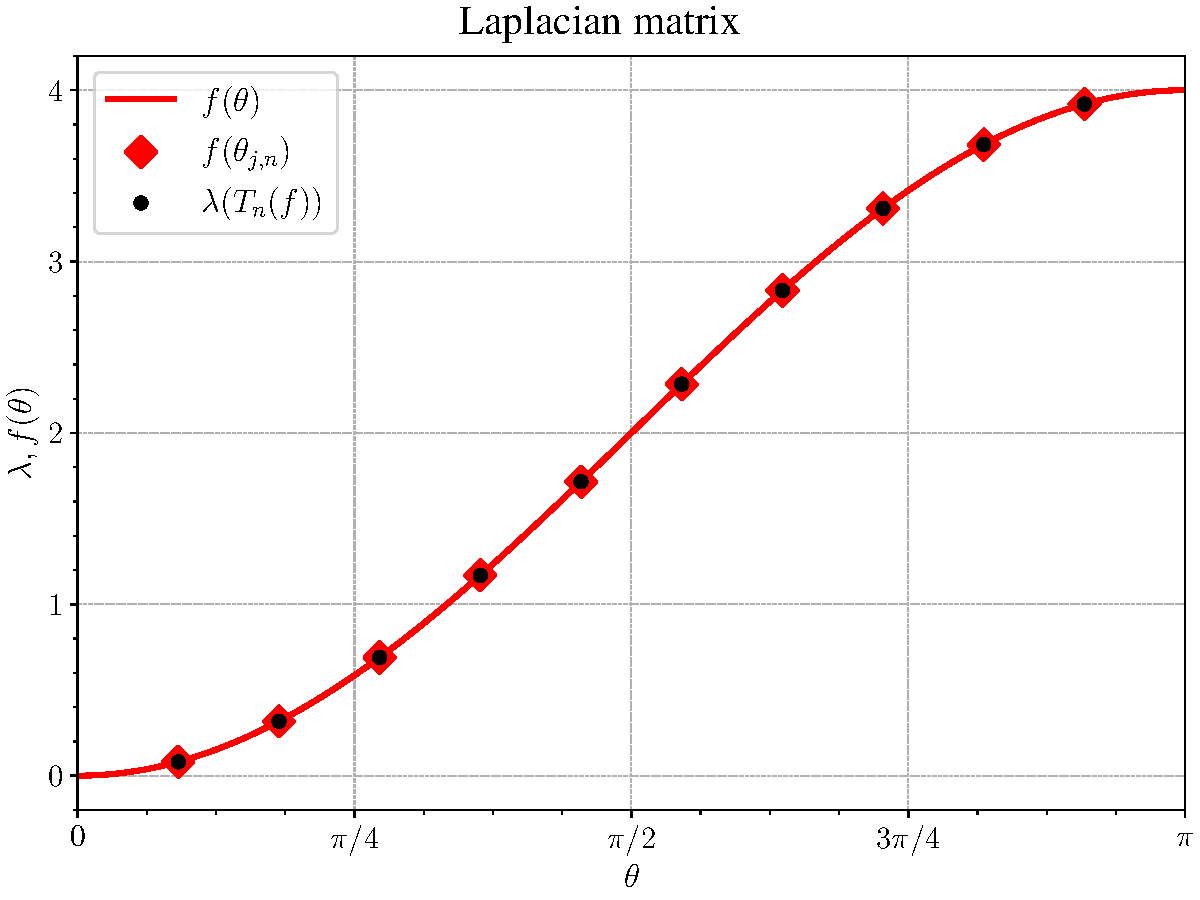
\includegraphics[width=0.7\linewidth]{images/Laplace_presentation.pdf}
        \caption{Symbolen $f(\theta)=2-2\cos(\theta)$, tillsammans med egenvärdena $\lambda(T_n(f))$. $\theta_{j,n}$ är ett s.k \textit{rutnät} definierad av $\theta_{j,n}=j\pi/(n+1)$, $n=10$.}
        % \label{fig:enter-label}
    \end{figure}
\end{frame}

\begin{frame}{Symbolic Regression}
\begin{itemize}
    \item En metod för att passa data till en funktion. \\
    \item Inom vanlig regression är funktionens struktur känd, man anpassar bara parametrar \\
    \item Inom SR görs inga antaganden för hur funktionen är uppbyggd
\end{itemize}
\end{frame}


\section{Metod}
\begin{frame}{Använda SR i Julia}
    \lstinputlisting[language=Python,basicstyle = \tiny\ttfamily, label=samplecode, caption=Example of code,
    %firstline=1, lastline=10
    ]{example_code.jl} 
\end{frame}

\begin{frame}{Preprocessing}
    Alla symboler är inte monotona%vilket innebär ...
    \begin{figure}[H]
    \centering
    \begin{subfigure}{0.49\textwidth}
        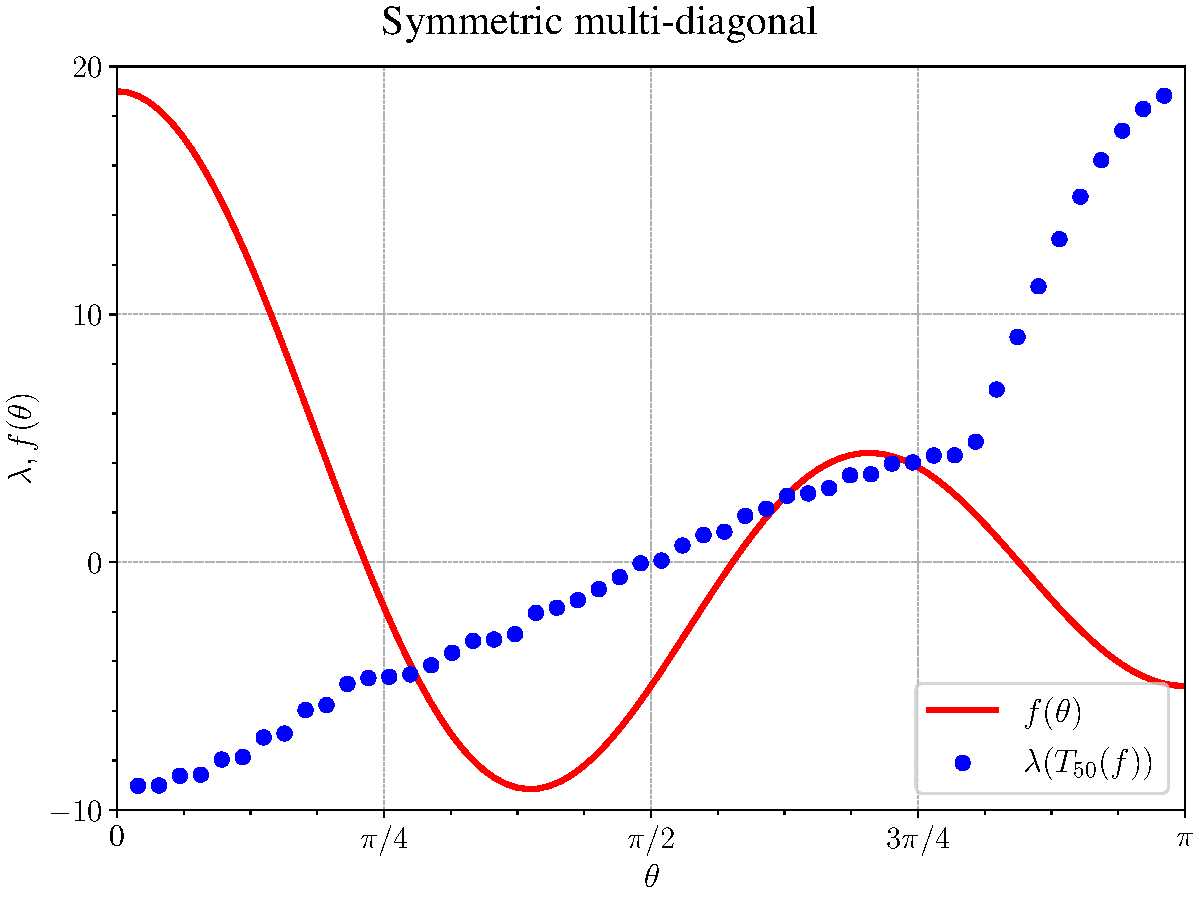
\includegraphics[width=\textwidth]{images/Preproc2unsorted.pdf}
        \caption{Icke-sorterade egenvärden}
        \label{fig:per_bi_lap_sym}
    \end{subfigure}
    \hfill
    \begin{subfigure}{0.49\textwidth}
        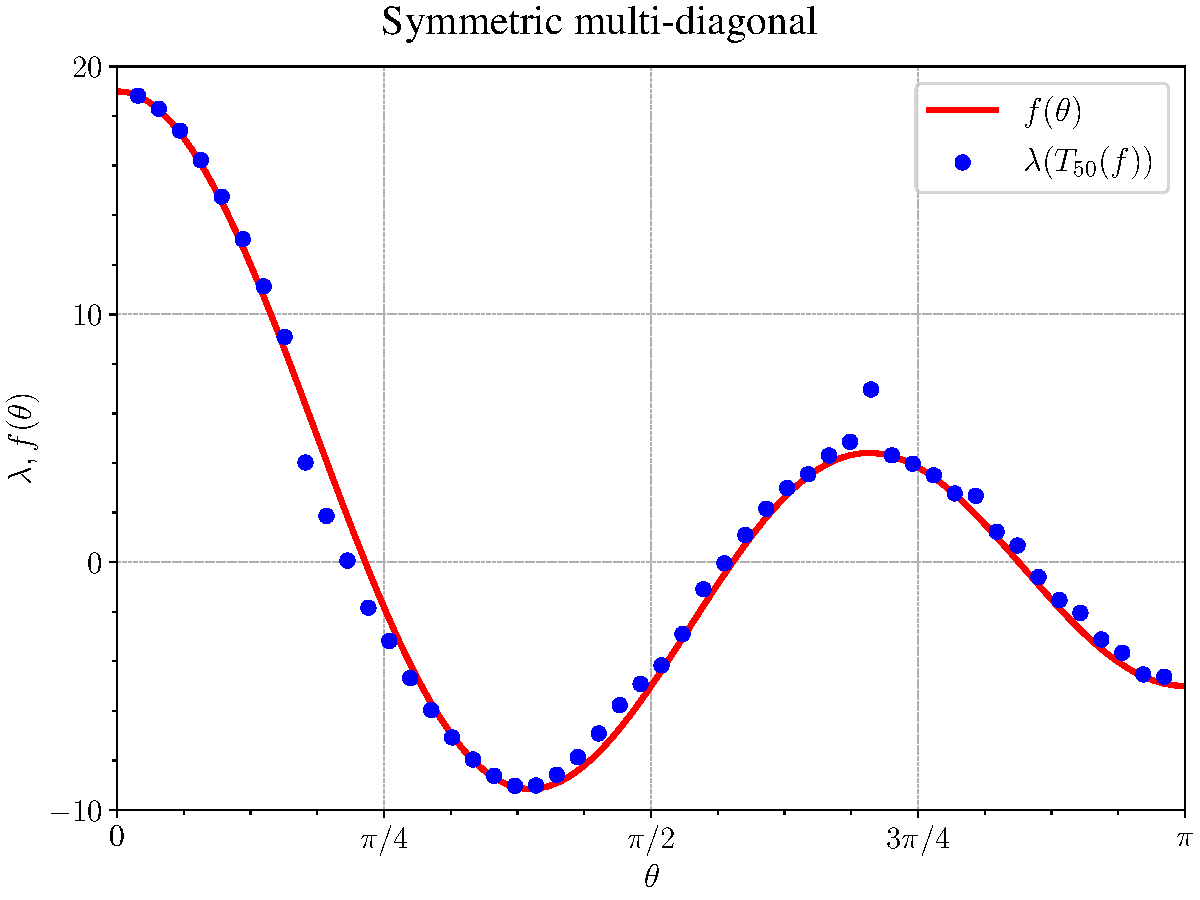
\includegraphics[width=\textwidth]{images/Preproc2sorted.pdf}
        \caption{Sorterade egenvärden}
        \label{fig:eigval_per_bilap}
    \end{subfigure}
    \caption{Spektrum av egenvärden förre och efter preprocessning för matris med $f(\theta)=1+4\cos(\theta)+6\cos(2\theta)+8\cos(3\theta)$}
    \label{fig:Spectrum Laplace & perturbed}
    \end{figure}
\end{frame}


\begin{frame}{Preconditioned Toeplitz}
    Preconditioning är vanligt inom beräkningsvetenskap när man vill sänka ``condition number" för att göra en numerisk metod mer stabil
\begin{equation}
T_n(g) = 
\begin{bmatrix}
3 & 1 &  &  \\
1 & \ddots&\ddots & \\
& \ddots &\ddots & 1\\
 &  & 1 & 3
\end{bmatrix}, \quad \text{``Preconditioner",}
\end{equation}
\begin{equation}
T_n(f) = 
\left[
\begin{array}{rrrrr}
4 & -1 & -1 & & \\
-1 & 4 & \ddots & \ddots & \\
-1 & \ddots & \ddots & \ddots & -1 \\
& \ddots & \ddots & 4 & -1 \\
& & -1 & -1 & 4
\end{array}
\right].
\end{equation}
\end{frame}

\begin{frame}{Preconditioned Toeplitz}
    \begin{equation}
T_6(g)^{-1}T_6(f) = 
\left[
\begin{array}{rrrrrr}
  1.6180  & -1       &  0       &  0       &  0       &  0.0027 \\
 -0.8541  &  2       & -1       &  0       &  0       & -0.0080 \\
 -0.0557   & -1       &  2       & -1       &  0       &  0.0212 \\
  0.0212  &  0       & -1       &  2       & -1       & -0.0557  \\
 -0.0080  &  0       &  0       & -1       &  2       & -0.8541 \\
  0.0027  &  0       &  0       &  0       & -1       &  1.6180 \\
\end{array}
\right],
\label{Precond example 6x6}
\end{equation}
Denna matris är väldigt lik Laplacianen, fast med perturberad ytterkolonner.
\end{frame}

\begin{frame}{Preconditioned}
    \begin{figure}[H]
    \centering
    \begin{subfigure}{0.49\textwidth}
        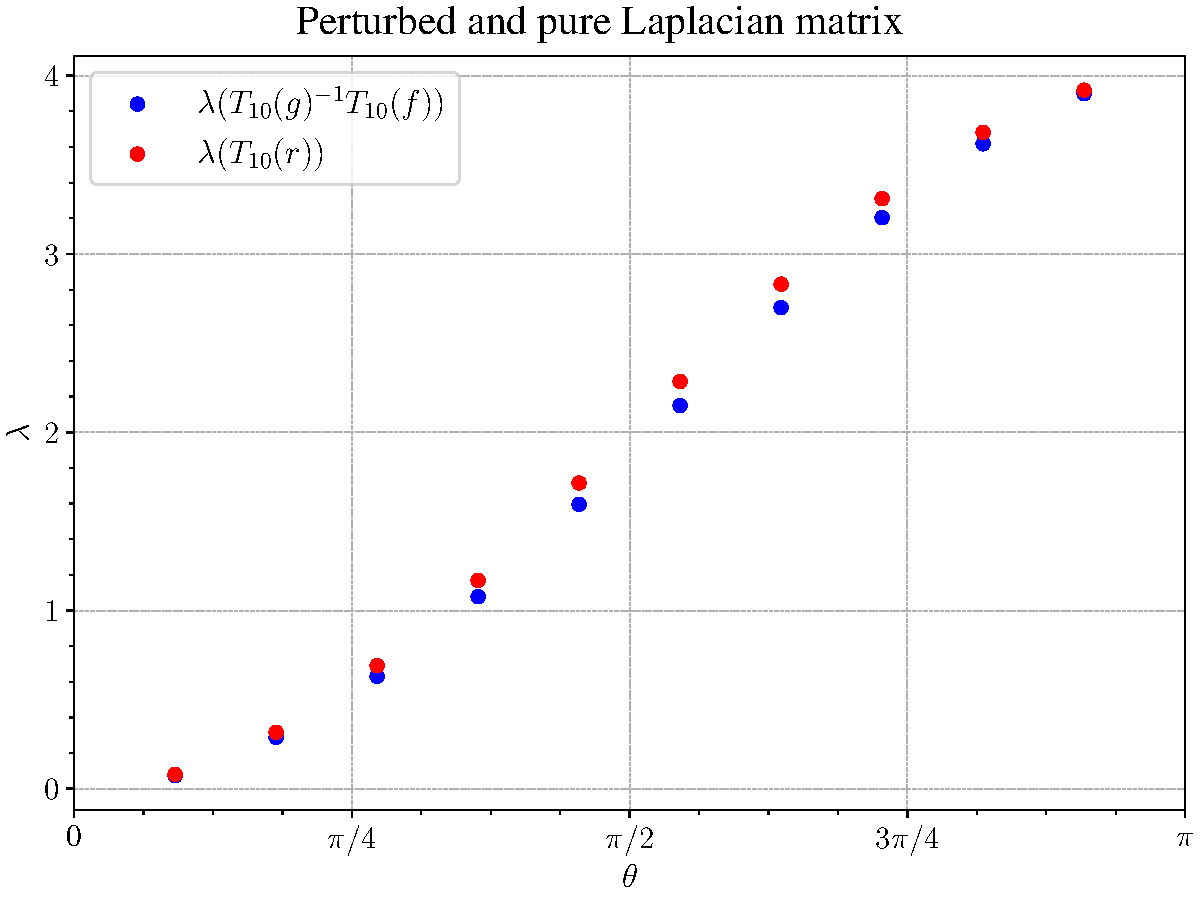
\includegraphics[width=\textwidth]{images/Precond_10.pdf}
        \caption{Eigenvalues of $10\times10$ Laplacian and perturbed Laplacian \eqref{Precond example 6x6}.}
        \label{fig:10x10 Laplacian & perturbed}
    \end{subfigure}
    \hfill
    \begin{subfigure}{0.49\textwidth}
        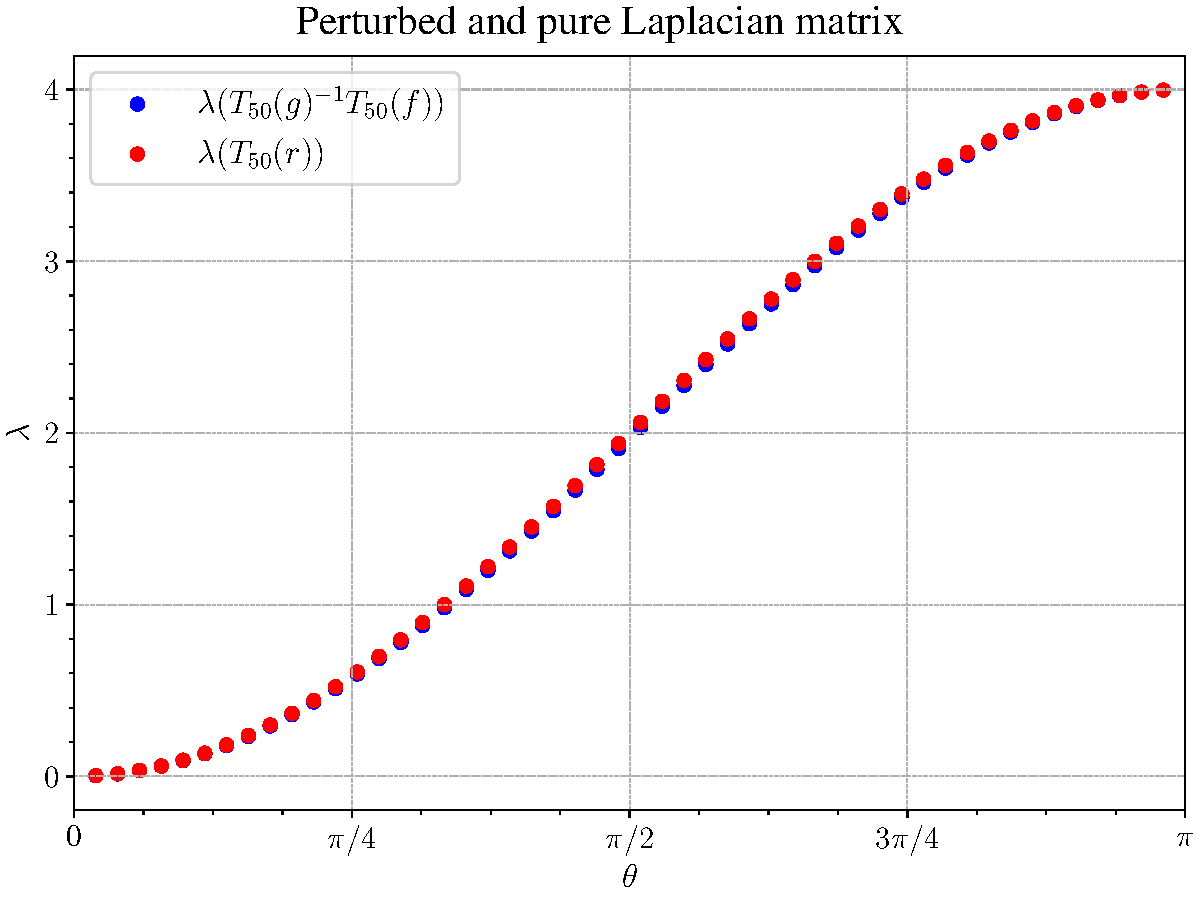
\includegraphics[width=\textwidth]{images/Precond_50.pdf}
        \caption{Eigenvalues of $50\times50$ Laplacian and perturbed Laplacian \eqref{Precond example 6x6}.}
        \label{fig:50x50 Laplacian & perturbed}
    \end{subfigure}
    \caption{Spectrum of Laplacian and perturbed Laplacian for sizes $n = 10,50$.}
    \label{fig:Spectrum Laplace & perturbed}
\end{figure}
\end{frame}

\begin{frame}{Block Toeplitz}
En block matris är en matris, där varje element också är en matris, man kan använda samma teori för Toeplitz matriser och symboler och skapa en s.k ``Block Toeplitz" 
\begin{equation}
    T_n(\mathbf{F}) = \begin{bmatrix}
        \hat{\mathbf{F}}_0 & \hat{\mathbf{F}}_1^T &\cdots & \hat{\mathbf{F}}_m^T \\ 
        \hat{\mathbf{F}}_1& \ddots&\ddots & & \ddots \\
        \vdots & \ddots &\ddots & \ddots & & \hat{\mathbf{F}}_m^T \\
        \hat{\mathbf{F}}_m & & \ddots& \ddots&\ddots & \vdots \\
        & \ddots &  & \ddots&\ddots&\hat{\mathbf{F}}_1^T \\
        & & \hat{\mathbf{F}}_m& \cdots & \hat{\mathbf{F}}_1&\hat{\mathbf{F}}_0
    \end{bmatrix},
    \label{eq: block-matrix template}
\end{equation}
\end{frame}

\begin{frame}{Block Toeplitz}
    \begin{equation}
    \hat{\mathbf{F}}_0=\begin{bmatrix}
    50 & 2 & 0 \\ 2 &-55 & 2 \\ 0 & 2 & 10
    \end{bmatrix}, \quad
    \hat{\mathbf{F}}_1 = \begin{bmatrix}
        11 & -1 & 0 \\ -1 & -6 & -1 \\ 0 & -1 &9
    \end{bmatrix}, \quad
    \hat{\mathbf{F}}_2 = \begin{bmatrix}
    1 & 0 & 2 \\ 0 & 1 & 0 \\2 & 0 & 1
    \end{bmatrix}
    \label{block-matrix entries}
\end{equation}
\end{frame}

\begin{frame}{Block Toeplitz}
    \begin{figure}
        \centering
        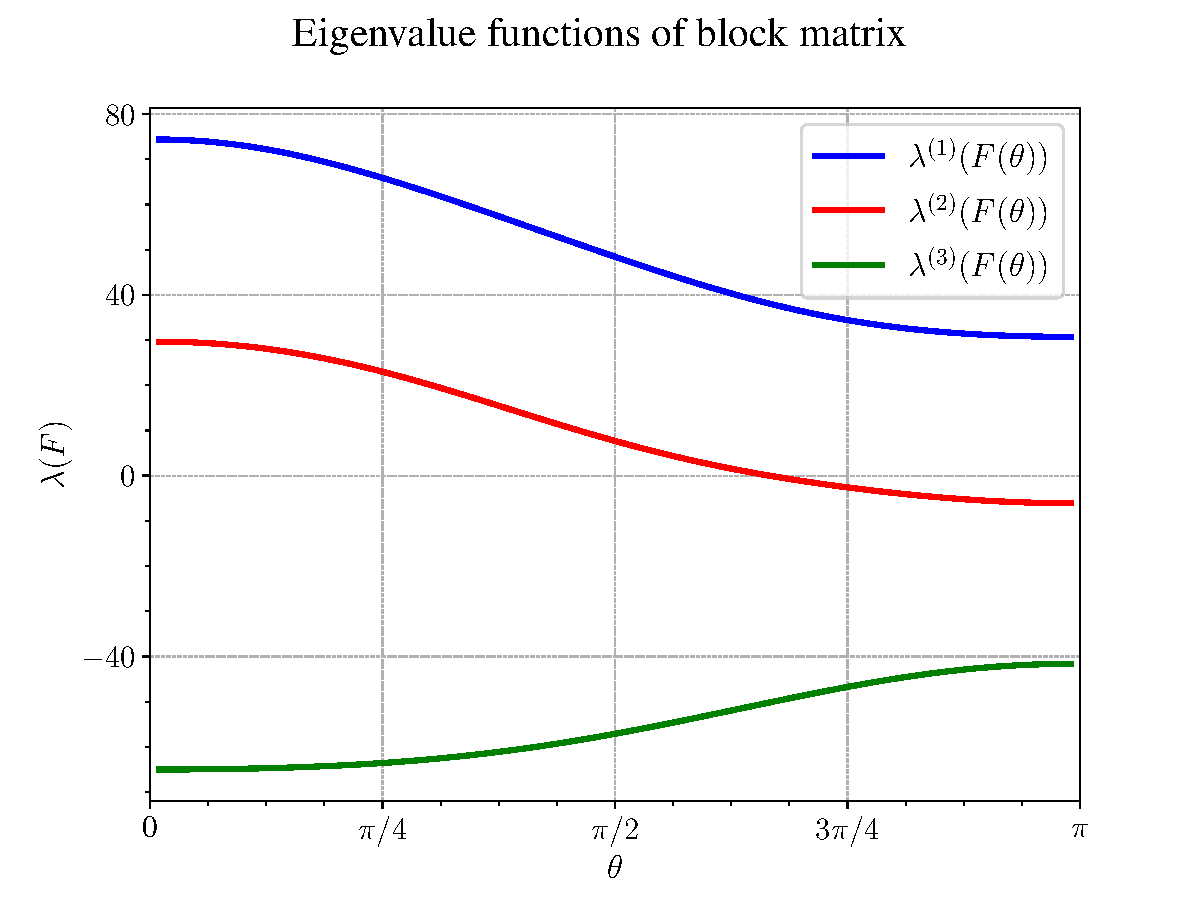
\includegraphics[width=0.7\linewidth]{images/Block_eigfunc.pdf}
        \caption{Eigenvalue functions of Block Toeplitz.}
        \label{Block eigfunc}
    \end{figure}
\end{frame}

% --------- SECTION 3 ------- %
% \begin{frame}{Förskjuten bi-Laplacian}
% Att ge SR tips
% \begin{equation*}
%     \scalebox{0.8}{$T_n(f)=
%     \begin{bmatrix}
%     -4 & 6 & -4 & 1&&\\
%     1&\ddots &\ddots & \ddots&\ddots  &\\
%     & \ddots&\ddots & \ddots&\ddots &1\\
%     &  & \ddots &\ddots&\ddots &-4\\
%     &  &  &\ddots  &\ddots&6\\
%     & & & & 1&-4
%     \end{bmatrix}, \quad f(\theta) = -4 + e^{i\theta} + 6e^{-i\theta} -4e^{-2i\theta} + e^{-3i\theta}$}
% \label{mat[-4,1][-4,6,-4,1]}
% \end{equation*}  
% \end{frame}

\begin{frame}{Okända matriser}
    \begin{figure}[H]
    \centering
    \begin{subfigure}{0.3\textwidth}
        \centering
        \[
        \scalebox{0.7}{$\begin{bmatrix}
        1 & 1 & 1 &1  \\
        -1&\ddots&\ddots&\ddots&\ddots\\
        % & \ddots&\ddots &\ddots &\ddots & \ddots&\\
        & \ddots&\ddots &\ddots  &\ddots &1\\
        & &\ddots & \ddots &\ddots &1\\
        &  & & \ddots& \ddots & 1\\
        & & &  & -1& 1
    \end{bmatrix}$}
        \]
        \caption{Grcar matrisen}
    \end{subfigure}
    \begin{subfigure}{0.3\textwidth}
        \centering
        \[
     \scalebox{0.7}{$\begin{bmatrix}
        0 & 3 & 1 &1 & \\
    -1&\ddots&\ddots&\ddots&\ddots\\
     %& \ddots&\ddots &\ddots &\ddots & \ddots&\\
     & \ddots &\ddots &\ddots &\ddots &1\\
     & &\ddots  & \ddots& \ddots&1\\
     &  & &\ddots  &\ddots &3\\
     & & & & -1& 0
        \end{bmatrix}$}
        \]
        \caption{Modifierad Grcar}
        \end{subfigure}
    \end{figure}
\end{frame}

\begin{frame}{Precision}
\begin{figure}[H]
    \centering
    \begin{subfigure}{0.49\textwidth}
        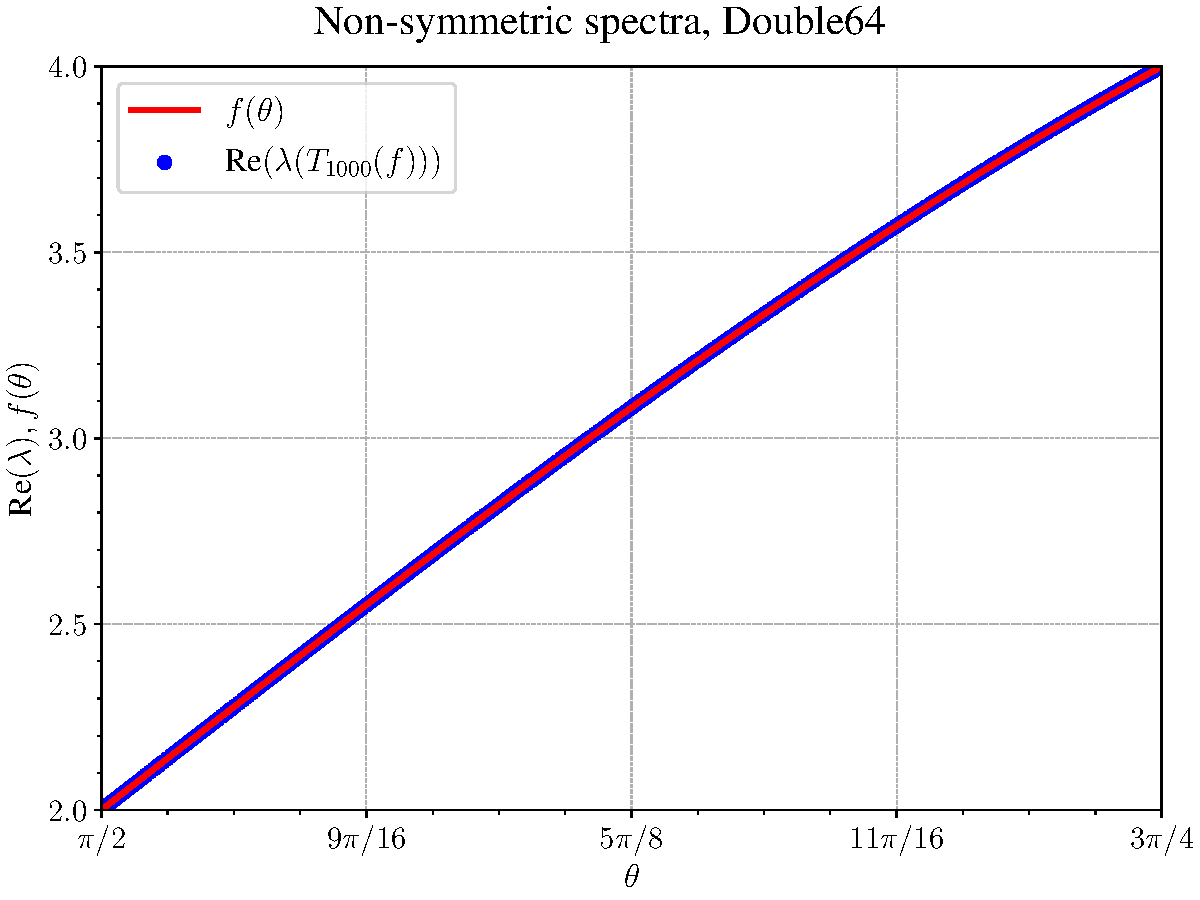
\includegraphics[width=\textwidth]{images/unstableeigDouble.pdf}
        \caption{\texttt{Double64}}
        \label{fig:per_bi_lap_sym}
    \end{subfigure}
    \hfill
    \begin{subfigure}{0.49\textwidth}
        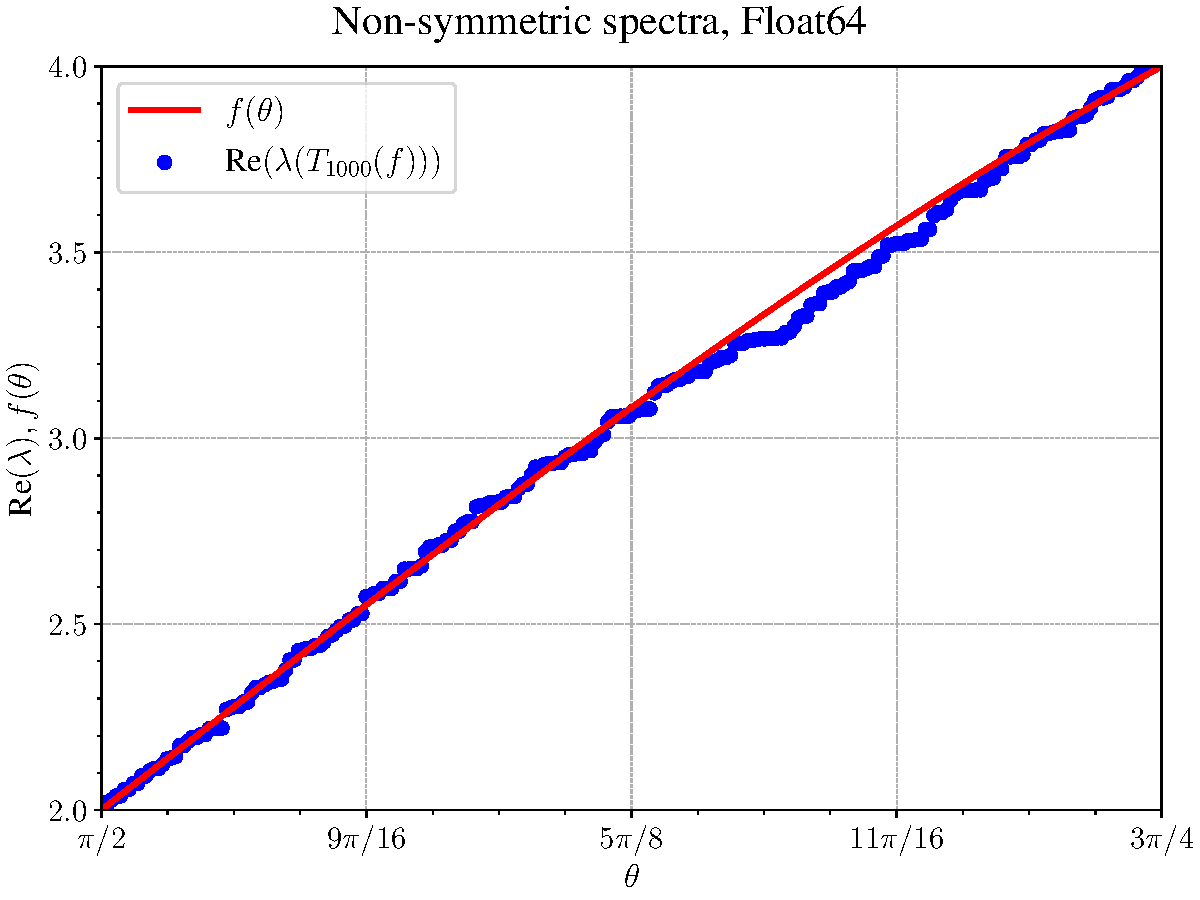
\includegraphics[width=\textwidth]{images/unstableeig.pdf}
        \caption{\texttt{Float64}}
        \label{fig:eigval_per_bilap}
    \end{subfigure}
    \caption{Spektrat för en $1000\times1000$ matris beräknat med olika noggrannhet.}
    \label{fig:Spectrum Laplace & perturbed}
    \end{figure}
\end{frame}

\begin{frame}{Grcar}
    Plottar man egenvärden för dessa matriser så ställer man sig snabbt frågan "hur ska egenvärdena vara ordnade?"
    \begin{figure}[H]
    \centering
    \begin{subfigure}{0.49\textwidth}
        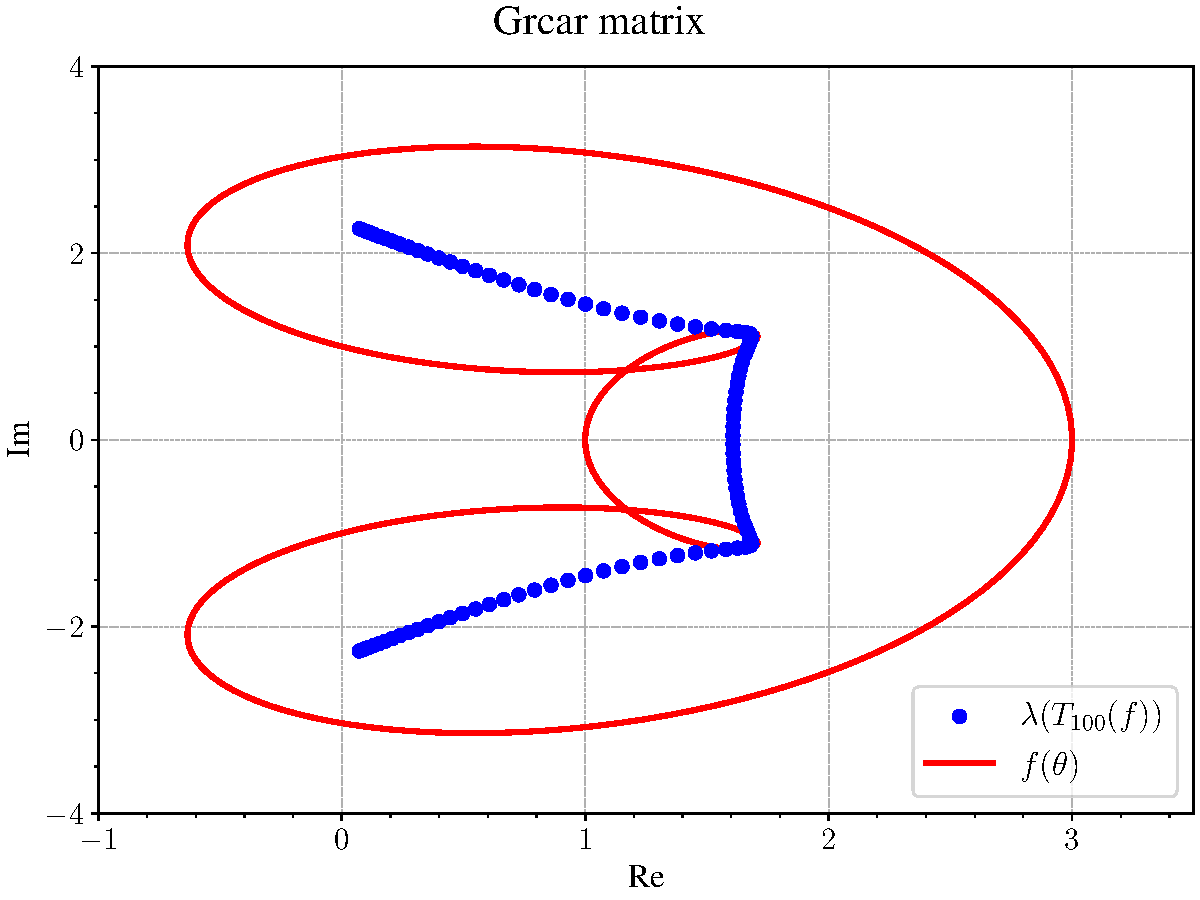
\includegraphics[width=\textwidth]{images/Grcar_comp.pdf}
        \caption{Grcar spektrum.}
        \label{fig:Grcar spectrum1}
    \end{subfigure}
    \hfill
    \begin{subfigure}{0.49\textwidth}
        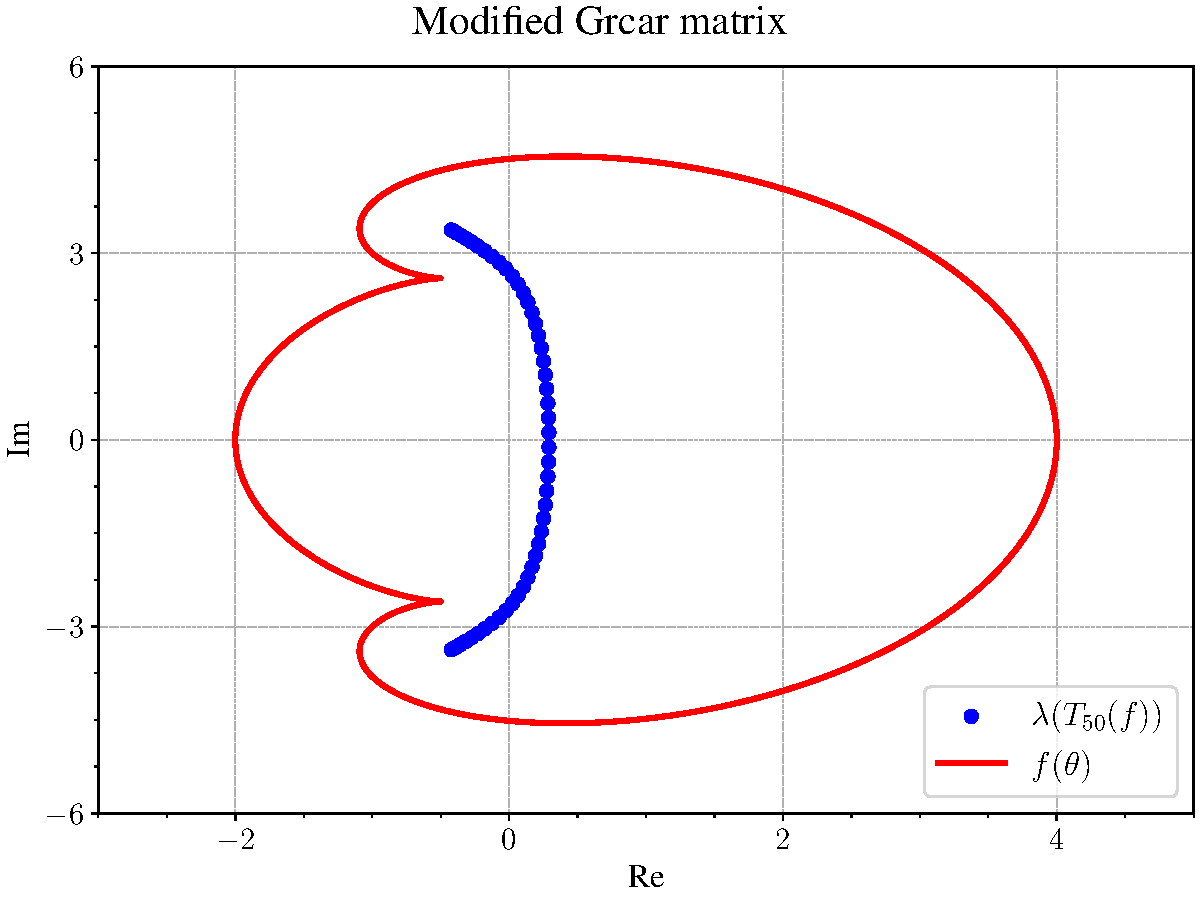
\includegraphics[width=\textwidth]{images/modifiedgrcar1comp.pdf}
        \caption{Modifierad Grcar spektrum.}
        \label{fig:Grcar spectrum2}
    \end{subfigure}
    \caption{Egenvärdena för Grcar-matriserna i komplexa talplanet}
    \label{fig:Grcar spektrum}
    \end{figure}
\end{frame}

\begin{frame}{Grcar}
Man kan sortera på en rad olika sätt
    \begin{figure}[H]
    \centering
    \begin{subfigure}{0.49\textwidth}
        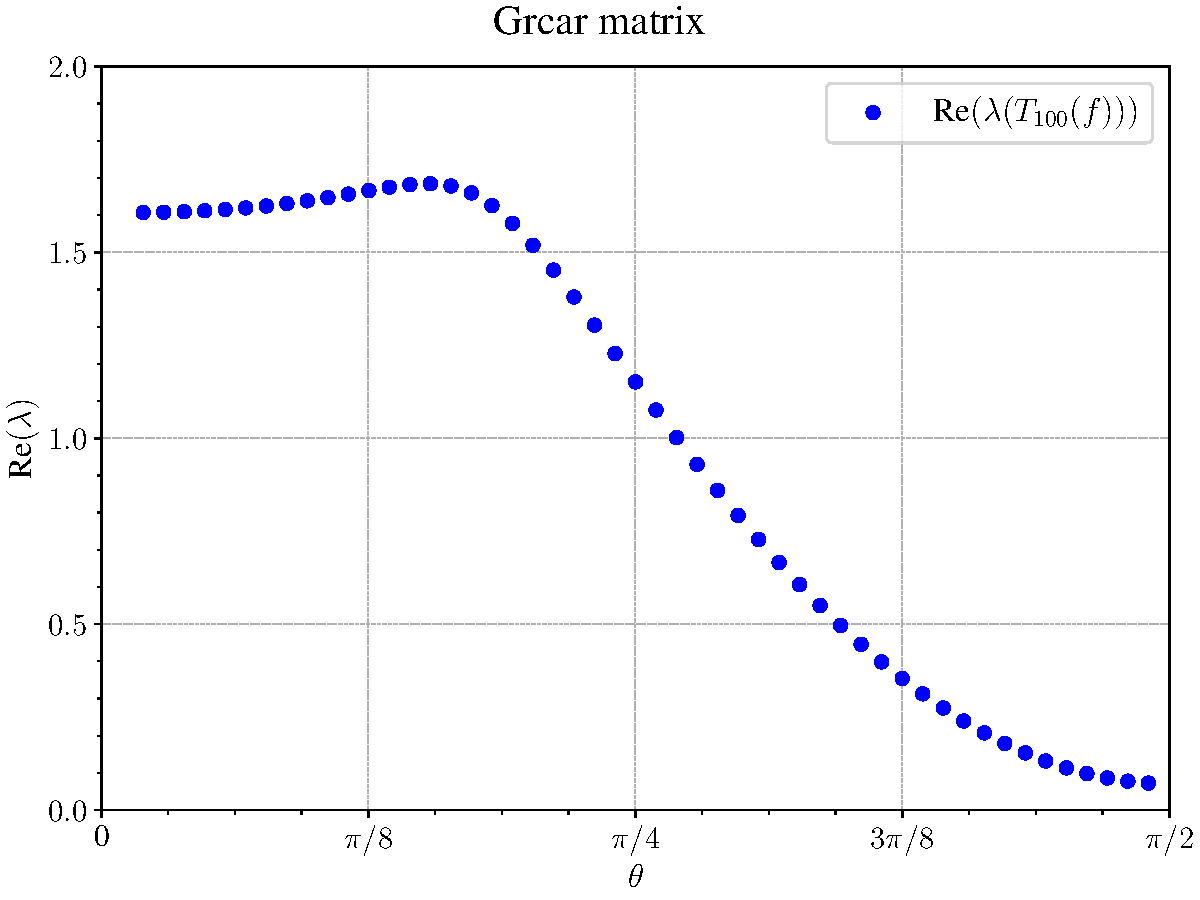
\includegraphics[width=\textwidth]{images/Grcar1.pdf}
        \caption{}
        \label{fig:Grcar sort1}
    \end{subfigure}
    \hfill
    \begin{subfigure}{0.49\textwidth}
        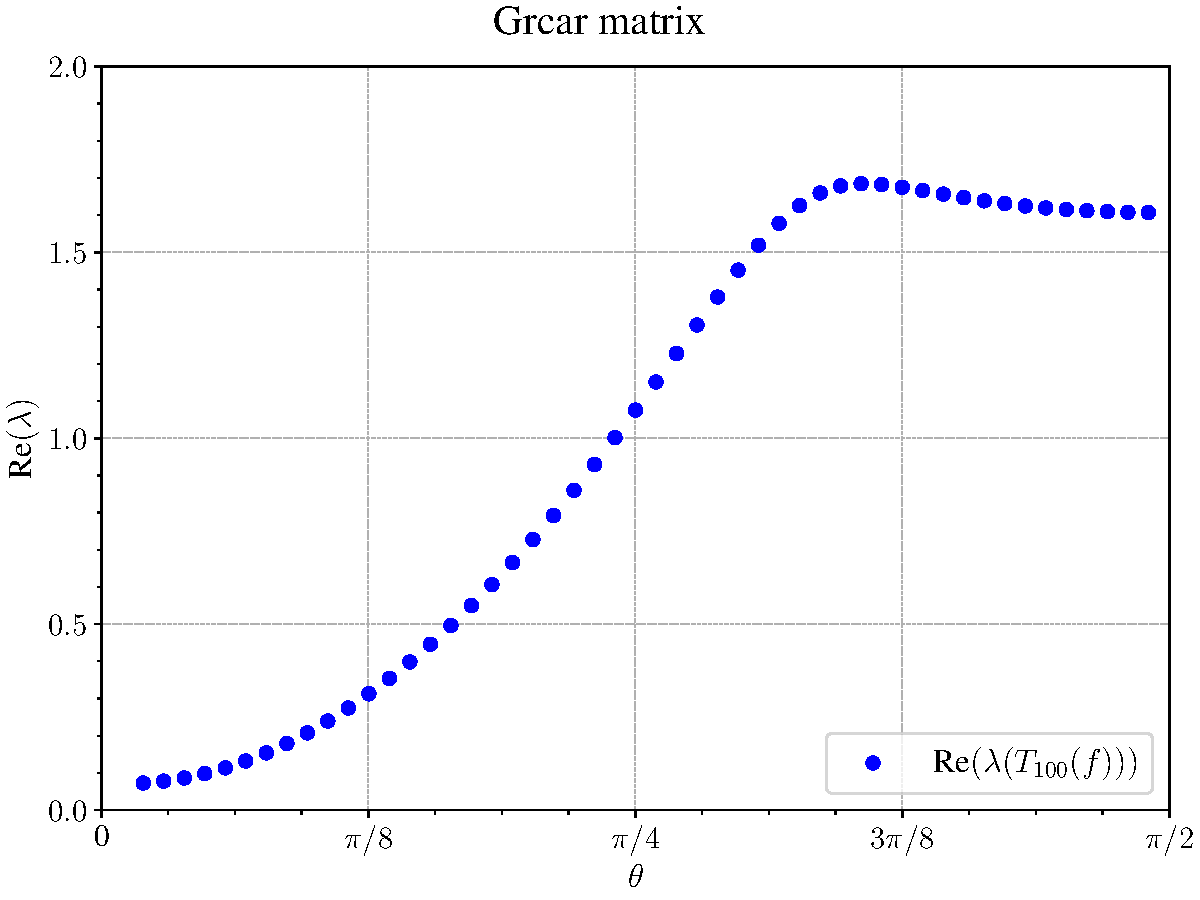
\includegraphics[width=\textwidth]{images/Grcar2.pdf}
        \caption{}
        \label{fig:Grcar sort2}
    \end{subfigure}
    \caption{Sorteringsalternativ 1}
    \label{fig:Sorteringsalternativ 1}
    \end{figure}
\end{frame}
\begin{frame}{Grcar}
    \begin{figure}[H]
    \centering
    \begin{subfigure}{0.49\textwidth}
        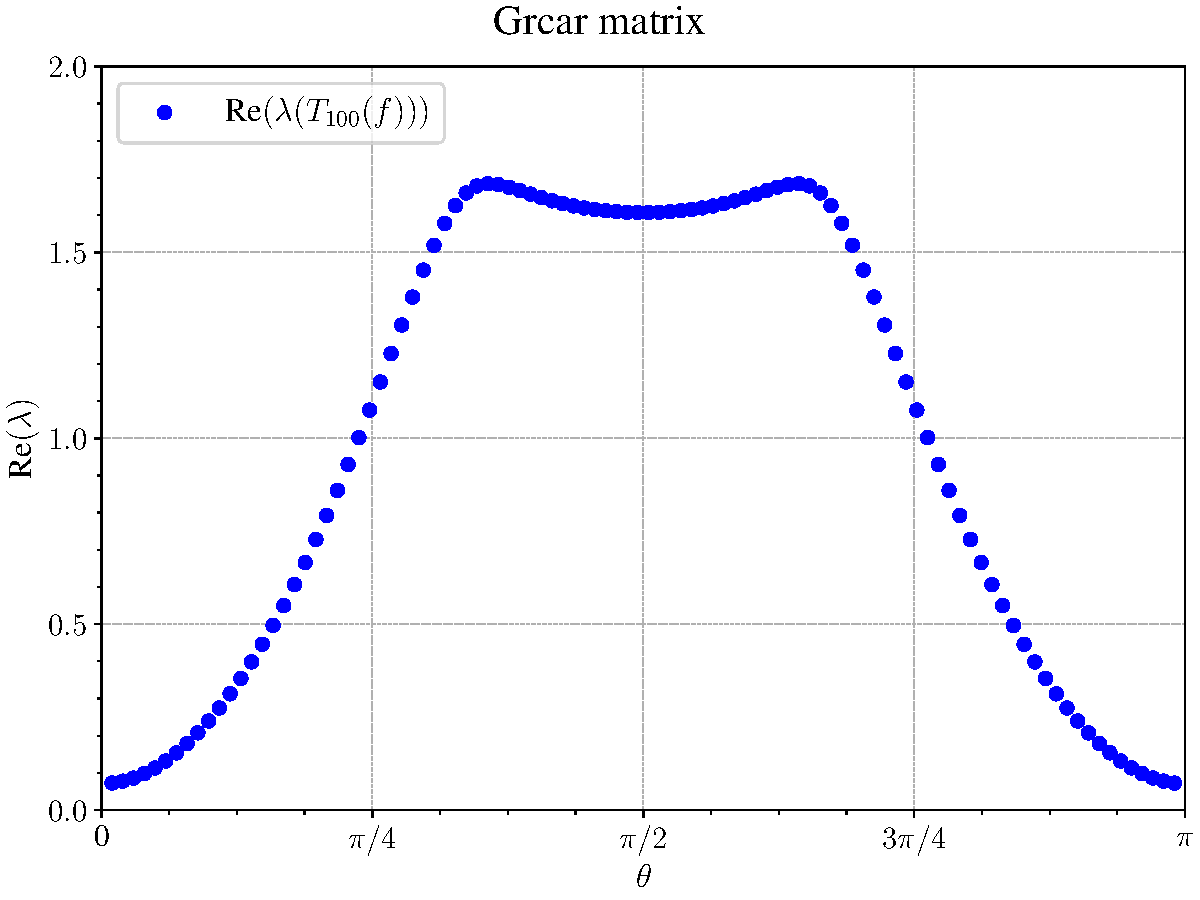
\includegraphics[width=\textwidth]{images/Grcar3.pdf}
        \caption{}
        \label{fig:Grcar sort3}
    \end{subfigure}
    \hfill
    \begin{subfigure}{0.49\textwidth}
        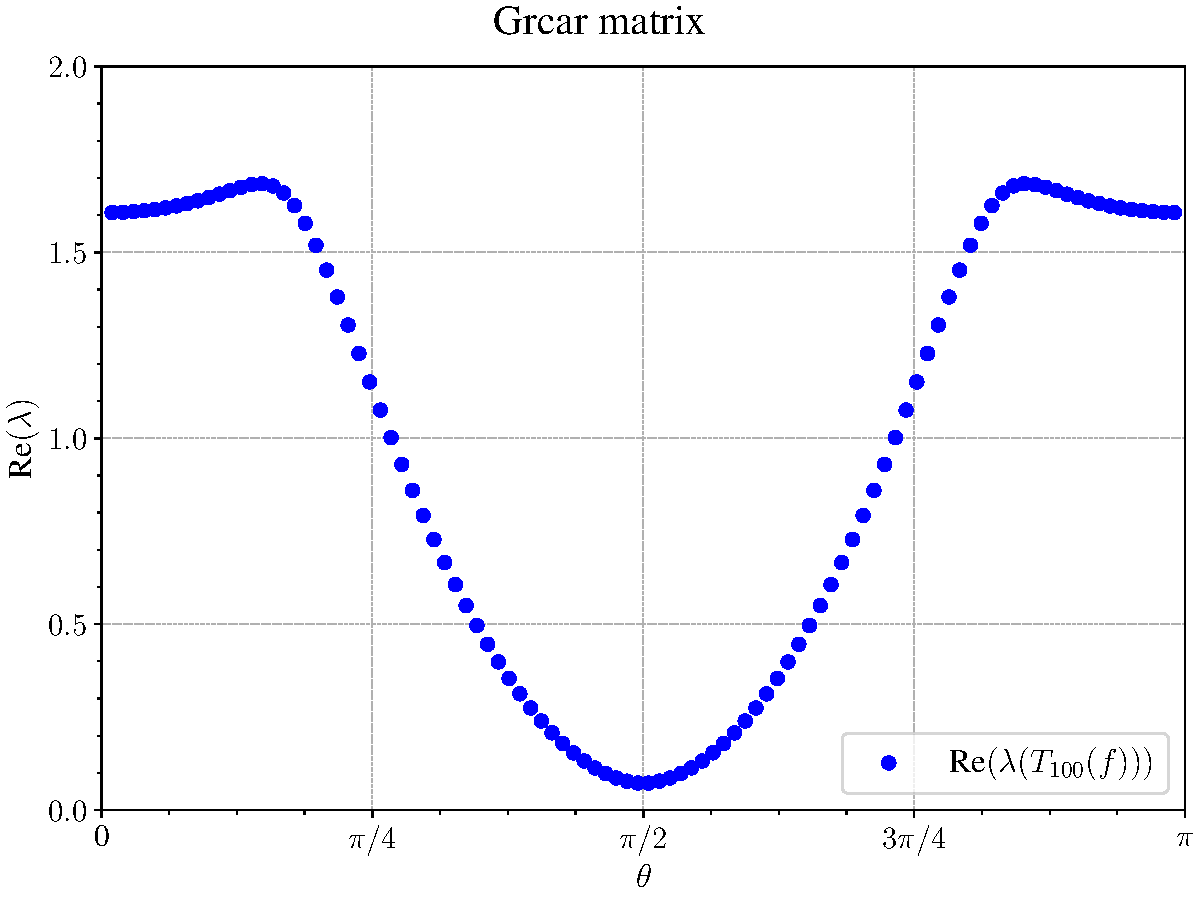
\includegraphics[width=\textwidth]{images/Grcar4.pdf}
        \caption{}
        \label{fig:Grcar sort4}
    \end{subfigure}
    \caption{Sorteringsalternativ 2}
    \label{fig:Sorteringsalternativ 2}
    \end{figure}
\end{frame}
% --------- SECTION 4 ------- %
\section{Resultat och diskussion}
\begin{frame}{Kända symmetriska matriser}
\begin{figure}[H]
    \centering
    \renewcommand{\arraystretch}{0.8}
    \begin{subfigure}{0.3\textwidth}
        \centering
        \scalebox{0.75}{$
        \begin{bmatrix}
        2 & -1 &        &        &   \\
       -1 & 2 & \ddots      &        &   \\
          & \ddots & \ddots & \ddots &   \\
          &        & \ddots     & 2      & -1 \\
          &        &        & -1     & 2
    \end{bmatrix}
    $}
        \caption{Laplacian}
    \end{subfigure}
    \begin{subfigure}{0.3\textwidth}
        \centering
        \scalebox{0.75}{$
     \begin{bmatrix}
        6  & -4 & 1      &        &   \\
       -4  & 6  & \ddots & \ddots &   \\
        1  & \ddots & \ddots & \ddots & 1 \\
           & \ddots & \ddots & 6      & -4 \\
           &        & 1      & -4     & 6
        \end{bmatrix}
    $}
        \caption{Bi-Laplacian}
        \end{subfigure}
        \begin{subfigure}{0.3\textwidth}
        \centering
        \scalebox{0.75}{$
        \begin{bmatrix}
            6  & -4 & 2      &        &   \\
       -4  & 6  & \ddots & \ddots &   \\
        2  & \ddots & \ddots & \ddots & 2 \\
           & \ddots & \ddots & 6      & -4 \\
           &        & 2      & -4     & 6
        \end{bmatrix}
        $}
        \caption{Störda bi-Laplacian}
    \end{subfigure}
    \caption{Symmetriska matriser.}
    \label{fig:sym_mats}
\end{figure}
\end{frame}

\begin{frame}{Kända Symmetriska matriser}
    \begin{columns}
        \column{0.3\textwidth}
        \textbf{Matris:}\\
        Laplacian\\
        Bi-Laplacian\\
        Störd bi-Laplacian
        \column{0.3\textwidth}
        \textbf{Symbol:}\\
        \scalebox{0.7}{$f(\theta) = 2-2\cos(\theta)$}\\
        \scalebox{0.7}{$g(\theta) = 6 - 8\cos(\theta) +2\cos(2\theta)$}\\
        \scalebox{0.7}{$h(\theta) = 6-8\cos(\theta)+4\cos(2\theta)$}
        \column{0.3\textwidth}
        \textbf{SR:}\\
        \scalebox{0.7}{$f(\theta) \approx 2-1.9998\cos(\theta)$}\\
        \scalebox{0.7}{$g(\theta) \approx 4(1 - cos(\theta))(1 - cos(\theta))$}\\
        \scalebox{0.7}{$h(\theta) \approx 2-8\cos(\theta)(1-\cos(\theta))$}
    \end{columns}
    \hfill
    \hfill
    \hfill
    \hfill
    \hfill
    \hfill
    
    \scalebox{0.7}{\textit{$\cos^2(\theta) = \frac{1}{2}\left( 1 + \cos(2\theta)\right)$}}
\end{frame}

\begin{frame}{Kända icke symmetriska matriser}
    \begin{figure}[H]
    \centering
    \begin{subfigure}{0.3\textwidth}
        \centering
        \[
        \begin{bmatrix}
        2 & 1 & & \\
        -1 & \ddots & \ddots & \\ 
        & \ddots & \ddots & 1 \\
        & & -1 & 2
    \end{bmatrix}
        \]
        \caption{}
    \end{subfigure}
    \begin{subfigure}{0.3\textwidth}
        \centering
        \[
     \begin{bmatrix}
        2 & i & & \\
        -i & \ddots & \ddots & \\
        & \ddots & \ddots & i \\
        & & -i & 2
        \end{bmatrix}
        \]
        \caption{}
        \end{subfigure}
        \begin{subfigure}{0.3\textwidth}
        \centering
        \[
        \begin{bmatrix}
            2 & -2 & & \\
            -1 & \ddots & \ddots & \\
            & \ddots & \ddots & -2 \\
            & & -1 & 2
        \end{bmatrix}
        \]
        \caption{}
    \end{subfigure}
    \\
    \caption{Namnlösa icke-symmetriska matrises.}
    \label{fig: Unnamed nonsym}
\end{figure}
\end{frame}

\begin{frame}{Kända icke symmetriska matriser}
    \begin{columns}
        \column{0.3\textwidth}
        \textbf{Matris:}\\
        (a)\\
        (b)\\
        (c)
        \column{0.3\textwidth}
        \textbf{Symbol:}\\
        \scalebox{0.7}{$f(\theta) = 2-2i\sin(\theta)$}\\
        \scalebox{0.7}{$g(\theta) = 2-2\sin(\theta)$}\\
        \scalebox{0.7}{$h(\theta) = 2 - 2\sqrt{2} \cos(\theta)$}
        \column{0.3\textwidth}
        \textbf{SR:}\\
        \scalebox{0.7}{$f(\theta) \approx 2 - 2i\sin(1.001\theta)$}\\
        \scalebox{0.7}{$g(\theta) \approx 2 -1.997\sin(\theta)$}\\
        \scalebox{0.7}{$h(\theta) \approx2 - 2.828\cos{(\theta)}$}
    \end{columns}
    \quad\quad\quad\quad\quad\quad\quad\quad\quad\quad\quad\quad\quad\quad\quad\quad\quad\quad\quad\quad\quad\quad\quad
    \scalebox{0.7}{\textit{$2\sqrt{2} \approx 2.828$}}
\end{frame}

\begin{frame}{Resultat: Förskjuten bi-Laplacian}
    \begin{columns}
        \column{0.4\textwidth}
        \scalebox{0.8}{$\begin{bmatrix}
        -4 & 6 & -4 & 1&&\\
        1&\ddots &\ddots & \ddots&\ddots  &\\
        & \ddots&\ddots & \ddots&\ddots &1\\
        &  & \ddots &\ddots&\ddots &-4\\
        &  &  &\ddots  &\ddots&6\\
        & & & & 1&-4
        \end{bmatrix}$}
        \\
        \textbf{Sanna symbol:}\\
        $f(\theta) = -\frac{\sin^4(\theta)}{\sin(\theta/4)\sin^3(3\theta/4)}$\\
        \column{0.6\textwidth}
        \textbf{Resultat med tips:}\\
        $ f_1(\theta) = \frac{\sin^4(1.596)\sin^4(\theta)}{\sin(0.249 \theta)\sin^3(-0.749\theta)}$\\
        $f_2(\theta) = \frac{\sin^3(\theta \cdot \sin^4(1.558))\sin(\theta)}{\sin( -0.249\theta)\sin^3(\theta \cdot \sin^4(1.196))}$\\
        \textbf{Resultat utan tips:}\\
        $f_3(\theta) = \frac{\frac{\sin^4(-0.998\theta) (-0.581 \cdot 1.697)}{\sin(0.247\theta)}}{\sin^3(0.7478\theta)}$\\
    \end{columns}
\end{frame}


\begin{frame}{Resultat :Förskjuten bi-Laplacian}
    Om man förenklar uttrycken
    
    \begin{columns}
        \column{0.4\textwidth}
        \textbf{Sanna symbolen:}\\
        \scalebox{0.75}{$f(\theta) = -\frac{\sin^4(\theta)}{\sin(\theta/4)\sin^3(3\theta/4)} \leftrightarrow$}\\
        \scalebox{0.75}{$f(\theta) =-\csc\left(\frac{\theta}{4}\right) \csc^3\left(\frac{3\theta}{4}\right) \sin^4(\theta)$}\\
        \column{0.6\textwidth}
        \textbf{Resultat med tips:}\\
        \scalebox{0.75}{$f_1(\theta) = -0.999 \csc(0.249\theta) \csc^3(0.749 \theta) \sin^4(\theta)$}\\
        \scalebox{0.75}{$f_2(\theta) = -\csc(0.249 \theta) \csc^3(0.7499\theta) \sin^3(0.9997 \theta) \sin(\theta)$}\\
        \textbf{Resultat utan tips:}\\
        \scalebox{0.75}{$f_3(\theta) =-1.445\csc^3(0.547046\theta)\sin(\theta)\sin^2(1.036\theta)$}\\
    \end{columns}
\end{frame}

\begin{frame}{Resultat: Preconditioned Toeplitz}
    \begin{figure}[H]
    \centering
    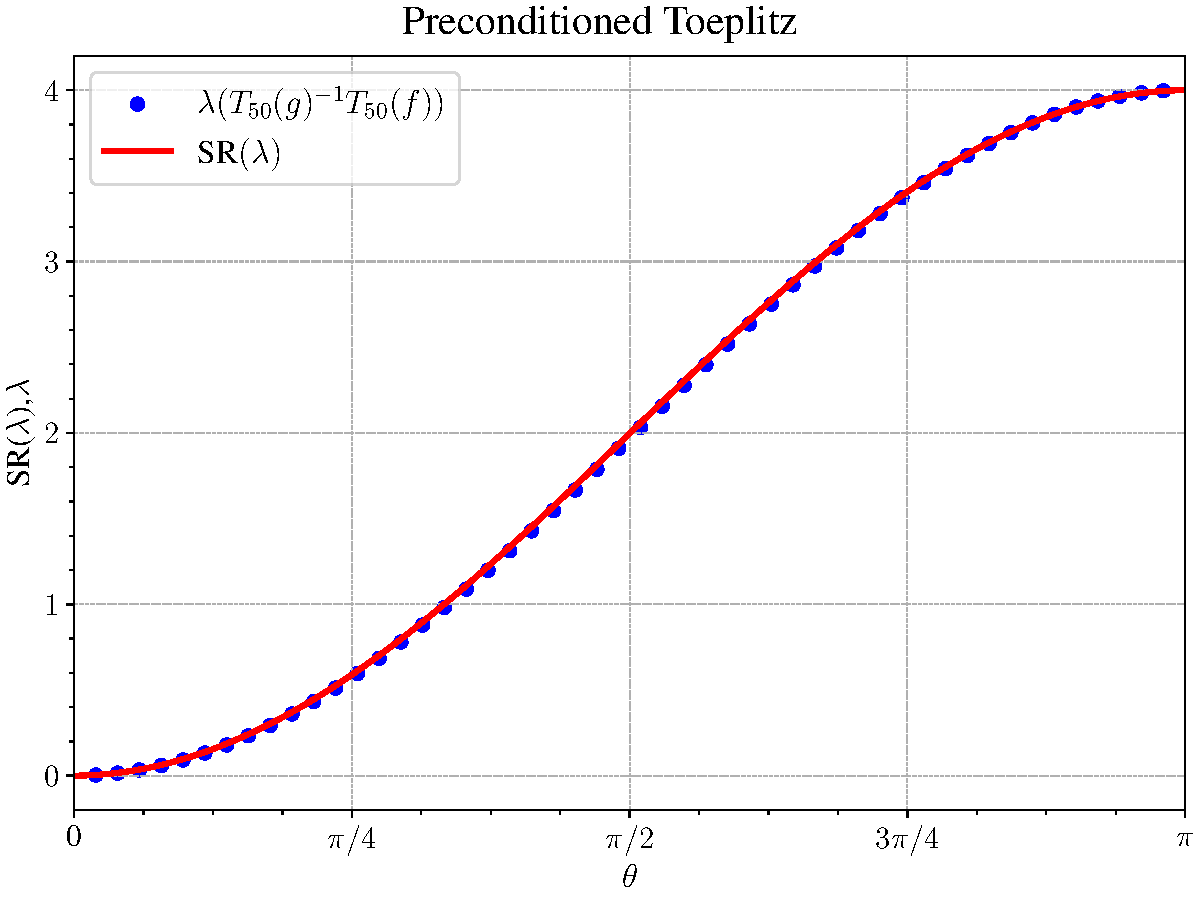
\includegraphics[width=0.5\linewidth]{images/Precondresults.pdf}
    \caption{Egenvärdena för preconditioned Toeplitx tillsammans med SR$(\lambda)$ \eqref{Results Preconditioned}.}
    \label{Preconditioned result}
\end{figure}
    \begin{align}    
        f(\theta)&=(\cos(\theta \cdot 1.933) \cdot (\theta \cdot 0.001)) + ((1.981 + (0.011 \cdot \theta)) 
        \\&- (\cos(\theta) \cdot 1.981)) \\
        & \approx 2 - 2\cos(\theta)
    \label{Results Preconditioned}
\end{align}

\end{frame}

\begin{frame}{Resultat: Block Toeplitz}
    \begin{figure}[H]
    \centering
    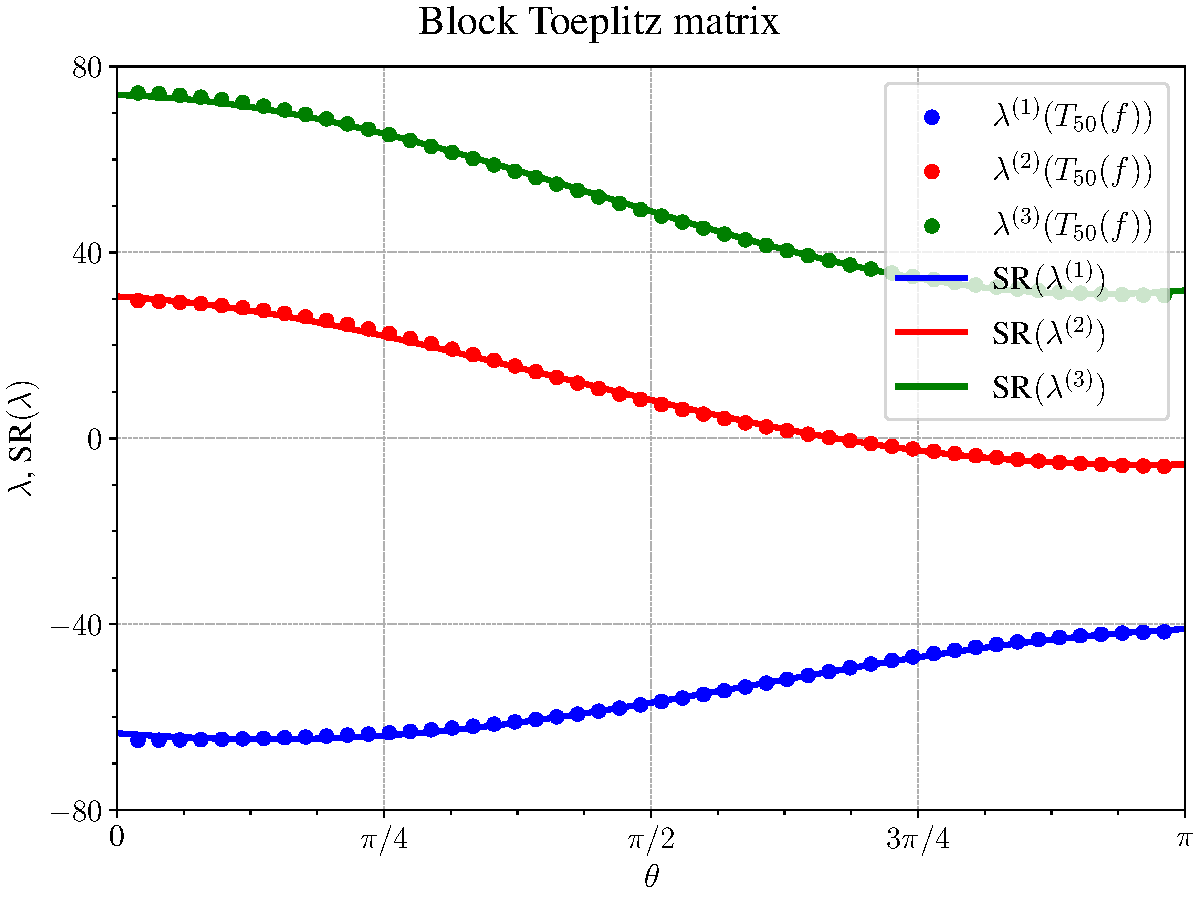
\includegraphics[width=0.5\linewidth]{images/Block_results.pdf}
    \caption{Results of SR Block Toeplitz.}
    \label{fig:Block Toepltix results}
    \end{figure}
\end{frame}
\begin{frame}{Resultat: Block Toeplitz}
    \begin{align}
    \text{SR}(\lambda^{(1)})=&(-4.6612 - \cos(\theta)) \cdot (\sin(\theta) + 11.2128),\label{eq: Block result 1}\\
    \text{SR}(\lambda^{(2)})=&(0.5152 + \cos(\theta)) \cdot ((\theta \cdot (-2.7095)) +20.1346),\label{eq: Block result 2}\\
    \text{SR}(\lambda^{(3)})=&((47.8922 - \theta) + (\theta^2)) - (\cos(\theta) \cdot (-25.9552 + \theta)).
    \label{eq: Block result 3}
    \end{align}
\end{frame}

\begin{frame}{Resultat: Grcar}
    \begin{figure}
    \centering
    \begin{subfigure}{0.49\textwidth}
        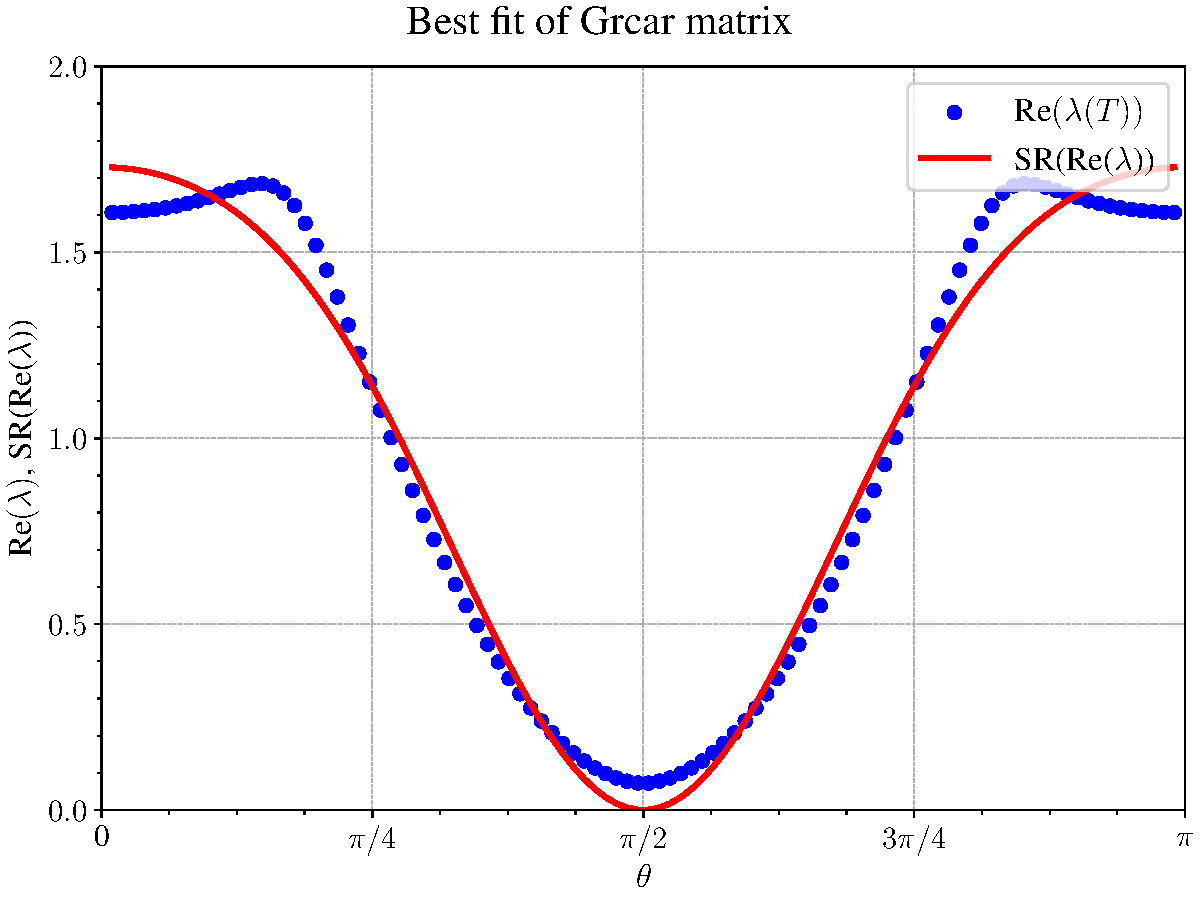
\includegraphics[width=\textwidth]{images/Ares1_re.pdf}
        \caption{Den reella delen av SR$(\lambda(T))$ tillsammans med $\lambda(T)$.}
        \label{fig:Ares1_re}
    \end{subfigure}
    \hfill
    \begin{subfigure}{0.49\textwidth}
        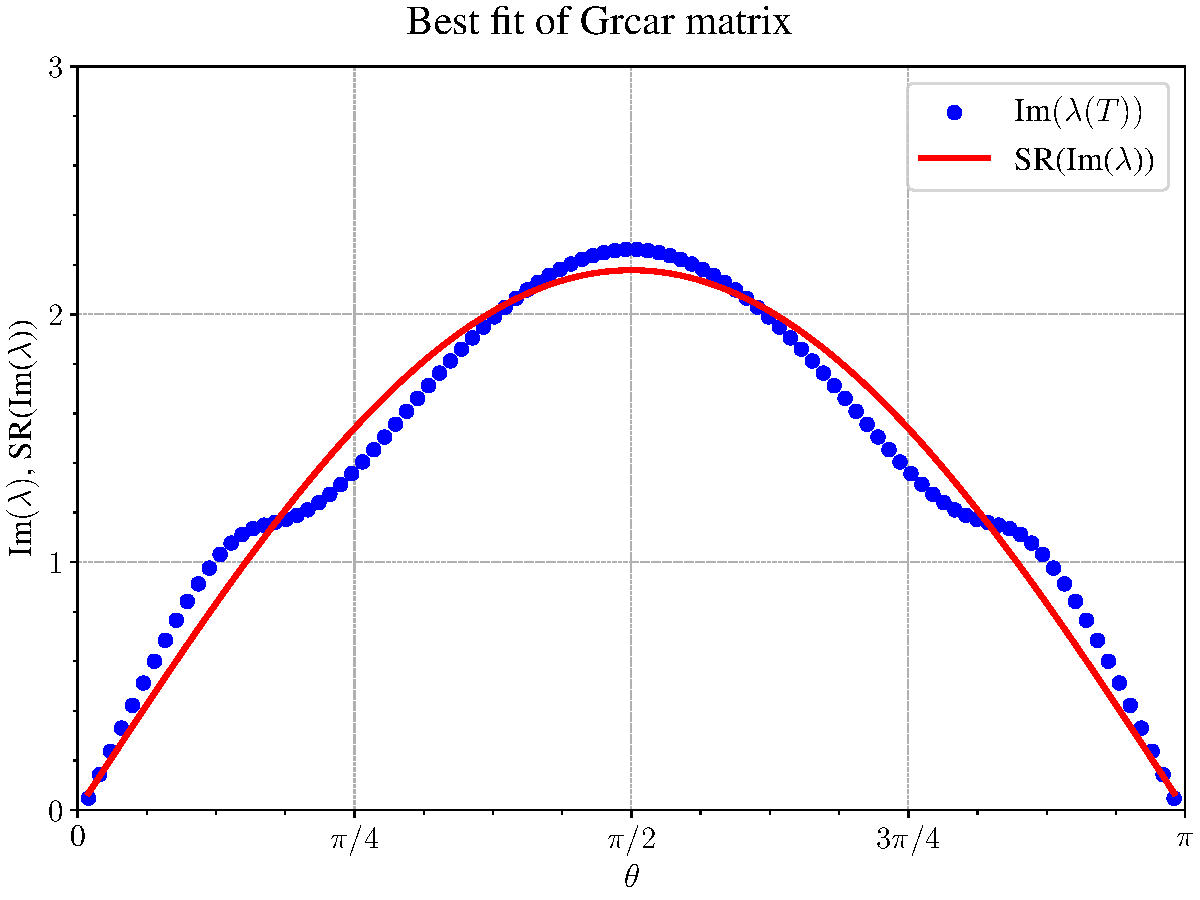
\includegraphics[width=\textwidth]{images/Ares1_im.pdf}
        \caption{Den imaginära delen av SR$(\lambda(T))$ tillsammans med $\lambda(T)$.}
        \label{fig:Ares1_im}
    \end{subfigure}
    \label{fig:Ares1}
    \caption{Reusltatet av SR för icke-modiferade Grcar matrisen, uppdelat på reella (vänster) och imaginära (höger) delen.}
    \end{figure}
\end{frame} 

\begin{frame}{Resultat: Modifierad Grcar}
\begin{align}
   &\begin{cases}
        \operatorname{Re}(f(\theta)) = 1.7394\cos(\theta)    \sin(1.679\cos(\theta))
        \\
        \operatorname{Im}(f(\theta)) = 2.178 \sin(\theta)
        \label{eq:Grcar1 A}
    \end{cases}
\end{align}
\end{frame}


\begin{frame}{Resultat: Modifierad Grcar}
 \begin{figure}[H]
    \centering
    \begin{subfigure}{0.49\textwidth}
        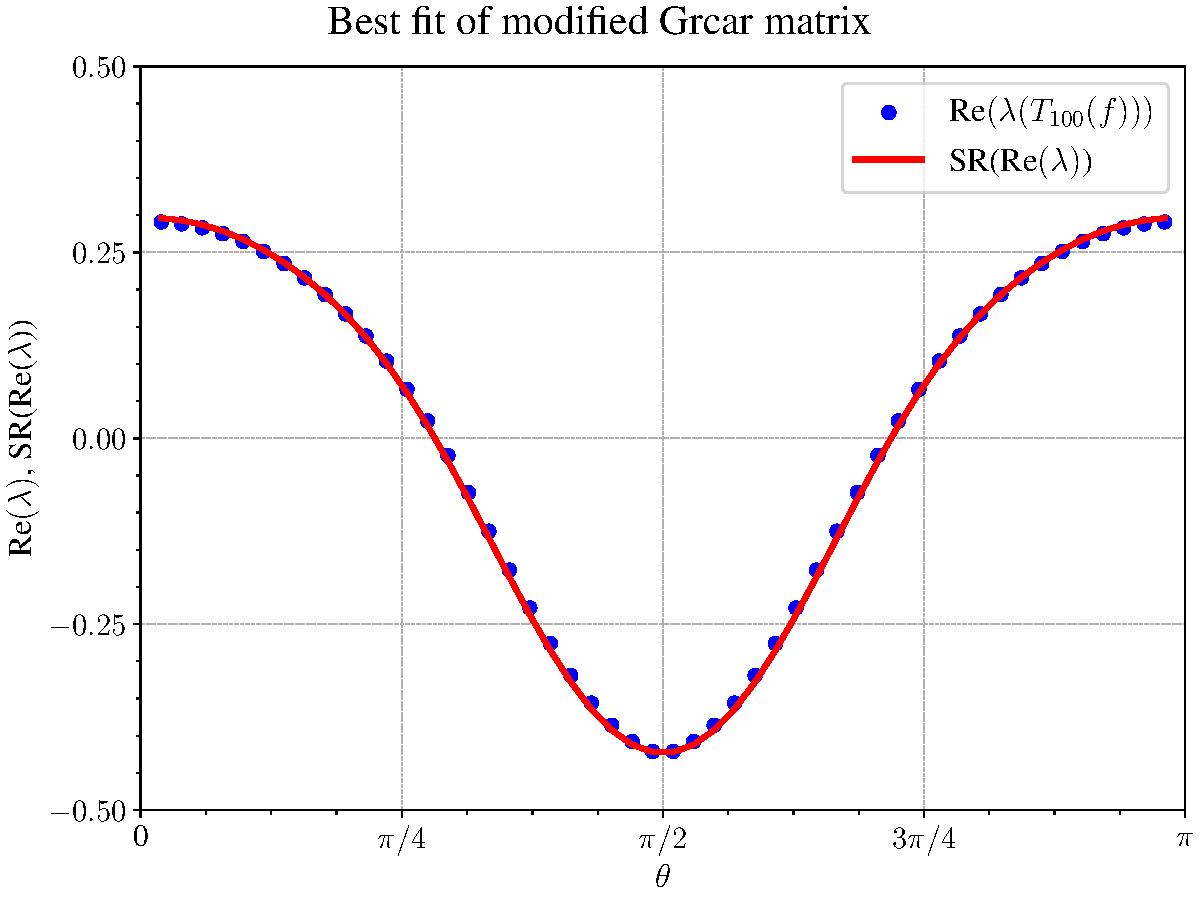
\includegraphics[width=\textwidth]{images/M_res2_re.pdf}
        \caption{Den reella delen av SR$(\lambda(T))$ tillsammans med $\lambda(T)$.}
        \label{fig:Mres2_re}
    \end{subfigure}
    \hfill
    \begin{subfigure}{0.49\textwidth}
        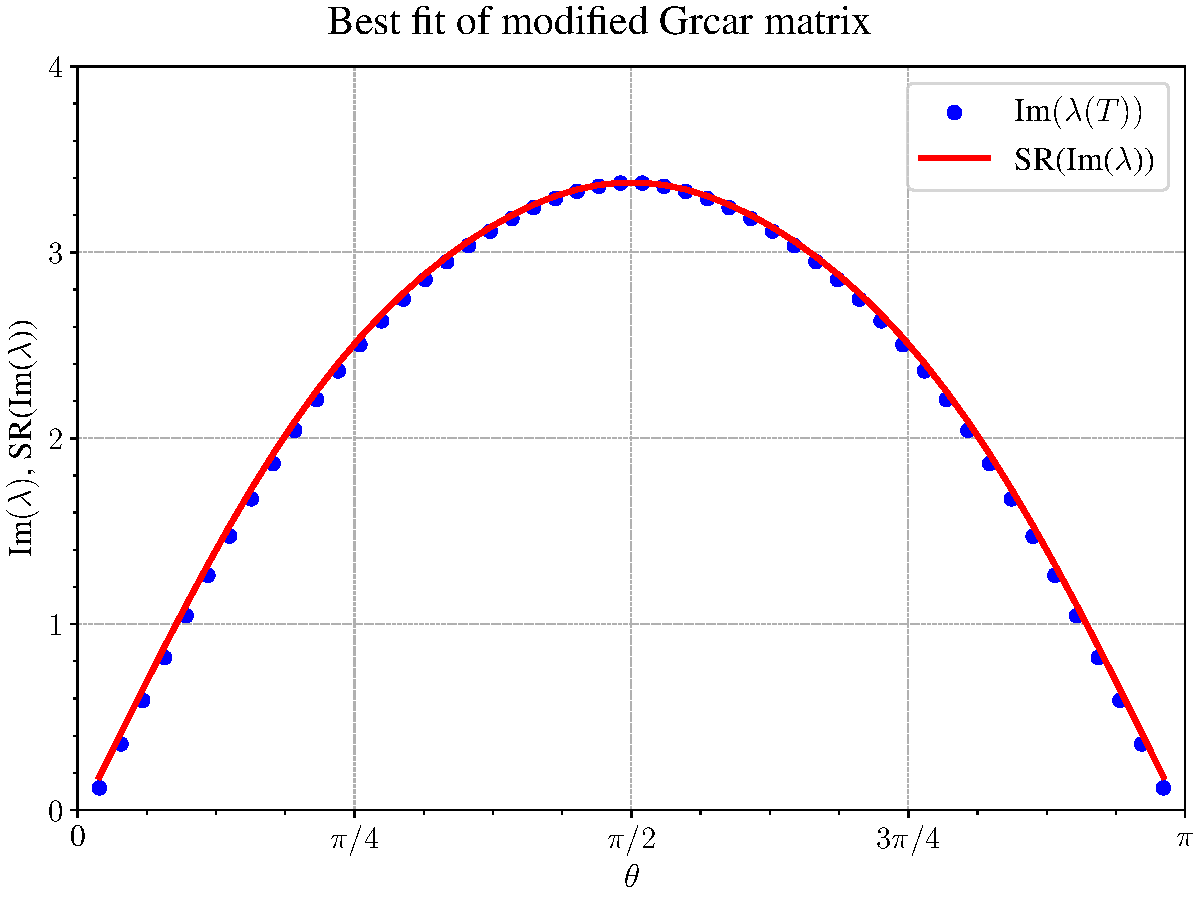
\includegraphics[width=\textwidth]{images/M_res2_im.pdf}
        \caption{Den imaginära delen av SR$(\lambda(T))$ tillsammans med $\lambda(T)$.}
        \label{fig:Mres2_im}
    \end{subfigure}
    \caption{Reusltatet av SR för modiferade Grcar matrisen, uppdelat på reella (vänster) och imaginära (höger) delen.}
    \label{fig:Mres2}
    \end{figure}
\end{frame}

\begin{frame}{Resultat Modifierad Grcar}
% \begin{figure}
%     \centering
%     \includegraphics[width=1\linewidth]{images/Screenshot 2025-05-28 at 14.10.26.png}
%     \caption{Caption}
%     \label{fig:enter-label}
% \end{figure}
\begin{align}
    &\begin{cases}
        \operatorname{Re}(f(\theta)) &=  0.38187 \cdot \sin\left( -\frac{0.59855 + \cos(\theta)}{0.38105} \right) - 0.03827\\
        &+  \cos\left( -\frac{\theta}{0.16675} - \cos\left( \theta -  2.11404 \cdot \cos(\theta) \right)  \right) \cdot 0.00334  
        \\
        \operatorname{Im}(f(\theta)) &= 0.15205 - \frac{2.89655 \cdot (\sin(\theta)-0.05484  )}{0.15047 - \sin(2.08197 - \cos(\cos(1.29655 \cdot \cos(\theta))))}
    \end{cases}
\label{eq:mod_g_2}
\end{align}
\end{frame}

\section{Slutsats}

\begin{frame}{Slutsats}
\begin{figure}
    \centering
    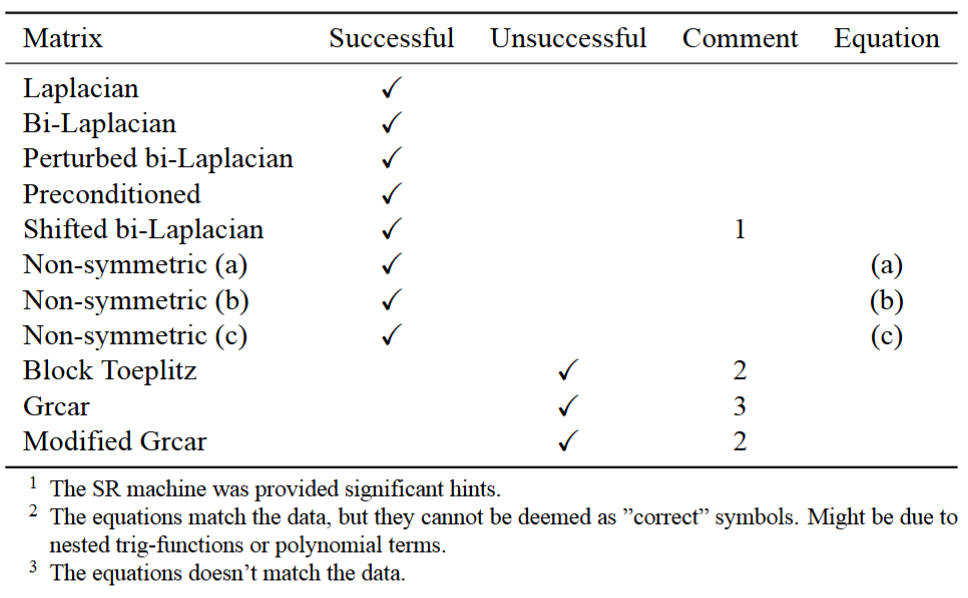
\includegraphics[width=0.9\linewidth]{images/BILD_AV_TABELL2.png}
    \caption{}
    \label{fig:enter-label}
\end{figure}
\end{frame}

% --------- SECTION 4 ------- %


\end{document}
